\documentclass[runningheads,a4paper]{llncs}

\usepackage{amssymb}
\usepackage{amsmath}
\usepackage{graphicx}
\usepackage[applemac]{inputenx} % This is required to support characters in spanish
\usepackage[T1]{fontenc} % This is required to have small-bold-capitals
\usepackage{fancyhdr} % This is required to have nice headers and footers
\usepackage{framed} % This is required to have framed comments
\usepackage{color} % This defines colors that can be used in the text
\usepackage{soul} % This allows the usage of \hl to highlight text
\usepackage{tocloft} % This is required to have custom lists of .....
\usepackage{comment} % This is required to remove specific environments
\usepackage{caption}
\usepackage{ifthen}
\usepackage{array}
\usepackage{wrapfig}
\usepackage{hyperref}
\usepackage{pifont}
\usepackage{listings}
\usepackage{syntax}
\usepackage{graphicx}
\usepackage{url}
\usepackage{latexsym}
\usepackage{fancybox}
\usepackage{pifont}
\usepackage{lineno}
\usepackage{todonotes}
\usepackage{multirow}
\usepackage{multicol}
\usepackage{xspace}
\usepackage{setspace}
\usepackage{todonotes}
\usepackage{bbding}
\usepackage{xcolor,colortbl}
\setcounter{tocdepth}{3}
\newtheorem{mydef}{Definition}


\newcommand{\mc}[2]{\multicolumn{#1}{c}{#2}}
\definecolor{Gray}{gray}{0.9}
\definecolor{LightGray}{gray}{0.98}

\newcolumntype{a}{>{\columncolor{Gray}}c}
\newcolumntype{b}{>{\columncolor{white}}c}

\newcommand\etal[0]{\emph{et al.}\xspace}
\newcommand\td[1]{\todo[inline]{#1}\xspace}

\setcounter{tocdepth}{3}


\urldef{\mailsa}\path|{david.mendez-acuna,jagalindo,benoit.combemale,benoit.baudry}@inria.fr|    
\newcommand{\keywords}[1]{\par\addvspace\baselineskip
\noindent\keywordname\enspace\ignorespaces#1}

\begin{document}

\mainmatter  % start of an individual contribution

\title{Reverse Engineering Language Product Lines}
\titlerunning{Reverse Engineering Language Product Lines}


\author{David M\'endez-Acu\~na \and Jos\'e A. Galindo \and Benoit Combemale \and Benoit Baudry}
\institute{University of Rennes 1, INRIA/IRISA. France\\
\vspace{1mm}\mailsa}
\authorrunning{David M\'endez-Acu\~na et. al}

\maketitle

\begin{abstract} 

The use of domain-specific languages (DSLs) is becoming a successful technique in the implementation of complex systems. However, the construction of this type of languages is time-consuming and requires highly-specialized knowledge and skills. Hence, researchers are currently seeking approaches to leverage reuse during the DSLs development in order to minimize implementation from scratch. An important step towards achieving this objective is to identify commonalities among existing DSLs. These commonalities constitute potential reuse that can be exploited by using reverse-engineering methods. In this paper, we present an approach intended to identify sets of DSLs with potential reuse. We also provide a mechanism that allows language designers to measure such potential reuse in order to objectively evaluate whether it is enough to justify the applicability of a given reverse-engineering process. We validate our approach by evaluating a large amount of DSLs we take from public \texttt{GitHub} repositories.

\end{abstract}

\section{Introduction}
\label{sec:introduction}

% Research context
The use of domain-specific languages (DSLs) has become a successful technique to achieve separation of concerns in the development of complex systems \cite{Cook:2006}. A DSL is a software language in which expressiveness is scoped into a well-defined domain that offers a set of abstractions (a.k.a., language constructs) needed to describe certain aspect of the system \cite{Combemale:2014}. For example, in the literature we can find DSLs for prototyping graphical user interfaces \cite{Oney:2012}, specifying security policies \cite{Lodderstedt:2002}, or performing data analysis \cite{Eberius:2012}.
 
\vspace{3mm}
Naturally, the adoption of such language-oriented vision relies on the availability of the DSLs needed for expressing all the aspects of the system under construction \cite{Clark:2013}. This fact carries the development of many DSLs which is a challenging task due the specialized knowledge it demands. A language designer must own not only quite solid modeling skills but also the technical expertise for conducting the definition of specific artifacts such as grammars, metamodels, compilers, and interpreters. As a matter of fact, the ultimate value of DSLs has been severely limited by the cost of the associated tooling (i.e., editors, parsers, etc...) \cite{jezequel:2014}.

To improve cost-benefit when using DSLs, the research community in software languages engineering has proposed mechanisms to increase reuse during the construction of DSLs. The idea is to leverage previous engineering efforts and minimize implementation from scratch \cite{Storm:2013}. These reuse mechanisms are based on the premise that ``software languages are software too'' \cite{Favre:2011} so it is possible to use software engineering techniques to facilitate their construction \cite{Kleppe:2009}. For instance, there are approaches that take ideas from Component-Based Software Engineering (CBSE) \cite{Cleenewerck:2003} and Software Product Lines Engineering (SPLE) \cite{Zschaler:2010} during the construction of new DSLs.

The basic principle underlying the aforementioned reuse mechanisms is that language constructs are grouped into interdependent \textit{language modules} that can be later integrated as part of the specification of future DSLs. Current approaches for modular development of DSLs (e.g., \cite{Vacchi:2015,Mernik:2013,Rumpe:2010}) are focused on providing foundations and tooling that allow language designers to explicitly specify dependencies among language modules as well as to provide the composition operators needed during the subsequent assembly process.

% Problem statement
Despite such important advances, the definition of language modules that can be actually useful in future DSLs is still a difficult task. This difficulty is due to several factors. For example, the reuse of a language module implies the reuse of all the constructs it offers; in many cases, some of those constructs are not necessary and, worst, they might be even conflictive. Language modules rarely can be reused `as-is' and without any adaptation. In this context, our research question is: \textit{How to define language modules that can be actually reusable in the construction of future DSLs?} %To answer that question language designers have to deal with several issues. For example, they have to find an appropriated level of granularity where, on one hand, language modules are fine enough so they contain small sets of constructs that are useful in several situations; on the other hand, language modules that are too small may over-complex the definition of DSLs so a good balance should be found. In addition, language designers need to find the correct combination of constructs that go well together.

Inspired in the work of Caldiera and Basili \cite{Caldiera:1991}, in this paper we propose a tool-supported approach that analyses a set of existing DSLs to extract a catalog of reusable language modules. The main idea is to perform static analysis on a given set of DSLs that are implemented in an homogeneous technology in order to detect groups of constructs that are typically used together. Once those groups are identified, we extract them by means of a break-down algorithm. Our approach considers not only syntax but also semantics of the DSLs under study. We validate our approach by applying it in an evaluation scenario with realistic DSLs that we obtain from public \textsc{GitHub} repositories. The results of this validation are quite promising.

%In this paper we propose an approach to leverage reuse during the construction of DSLs focused on legacy DSLs. In other words, we propose to exploit reuse in existing DSLs that are were not necessarily built for being reused but that share some commonalities (i.e., they provide similar language constructs). In particular, we present an strategy to identify groups of constructs that are frequently used together in a given sets of legacy DSLs. Then, a catalog of language modules is extracted from the commonalities by means of a reverse-engineering method. To do so, we perform static analysis on the artifacts where the DSLs are specified and compare language constructs at the level of the syntax and semantics.

The reminder of this paper is organized as follows: Section \ref{sec:background} introduces a set of preliminary definitions/assumptions as well as an illustrating scenario that we use all along the paper. Section \ref{sec:apprach} describes our approach that is evaluated in Section \ref{sec:validation}. Section \ref{sec:relatedwork} presents the related work and, finally, Section \ref{sec:conclusions} concludes the paper. 

%The aforementioned reuse mechanisms can be adopted by means of two different approaches: \textit{top-down} and \textit{bottom-up}. The top-down approach proposes the design and implementation from scratch of reusable language modules that can be employed in the construction of several DSLs. Differently, the bottom-up approach proposes the use or reverse-engineering processes to extract those language modules from existing DSLs that share some commonalities which can be properly encapsulated. Whereas the major complexity in top-down approaches is that language designers should design language modules by trying to predict their potential reuse; bottom-up approaches do not have to deal with that problem. Rather, the extraction of the reusable language modules is based on the detection of commonalities in existing DSLs. Consequently, bottom-up approaches can be considered as promising approach and, indeed, there are already in the literature some works (e.g., \cite{vacchi:2014}) advancing towards that direction. 

%The success of this strategy relies on a set of design decisions that favor extensibility and/or genericity thus increasing the probabilities that the language modules are useful in the future. In this case, the major complexity comes from the fact that language designers do not know \textit{a priori} the needs of future DSLs. Consequently, in practice many of these building blocks are not reusable \textit{as is} and rather they require some previous adaptation.

% Contribution


%It is quite important to mention that our approach is inspired on the work of Berger et al X that presents the foundations for measuring product line-ability of families of software products in the general case. Our contributions with respect to that work are that we apply these ideas to the particular case of DSLs. Besides, at the best of our knowledge, there is not a tool implementing such ideas so we introduce a proposal. Finally, we apply our proposal in an empirical study performed on GitHub repositories where the objective is to identify families of DSLs in the Web and to evaluate its potential reuse. 

% Outline


%Despite such important advances, the definition of language modules that can be actually useful in future DSLs is still a difficult task. In part, this difficulty is due to the fact that the reuse of a language module implies the reuse of all its constructs and language designers do not always have the information that allow them to predict the correct combination of constructs that go well together. What is the correct level of granularity? Are there constructs that should be always together? Are there constructs that should be always separated?
\section{Problem statement}
\label{sec:problem}
\section{Proposed approach}
\label{sec:approach}

\subsection{Overview}

\subsection{Breaking down the DSLs}

The objective of this step is to divide the DSL in several language modules that can be latter composed. To do so, we need to deal with two problems. The former is to find the way in which the we will split the language constructs. The second one is to define the language modules themselves with their corresponding required and provided interfaces. 

\subsubsection{Identifying constructs distribution}

The input is the set of DSLs. We first identify the language constructs for each one. Then we perform a match according to a given comparison operator. Then, we merge. Finally, we execute a graph partitioning algorithm. 

\begin{figure*}
\centering
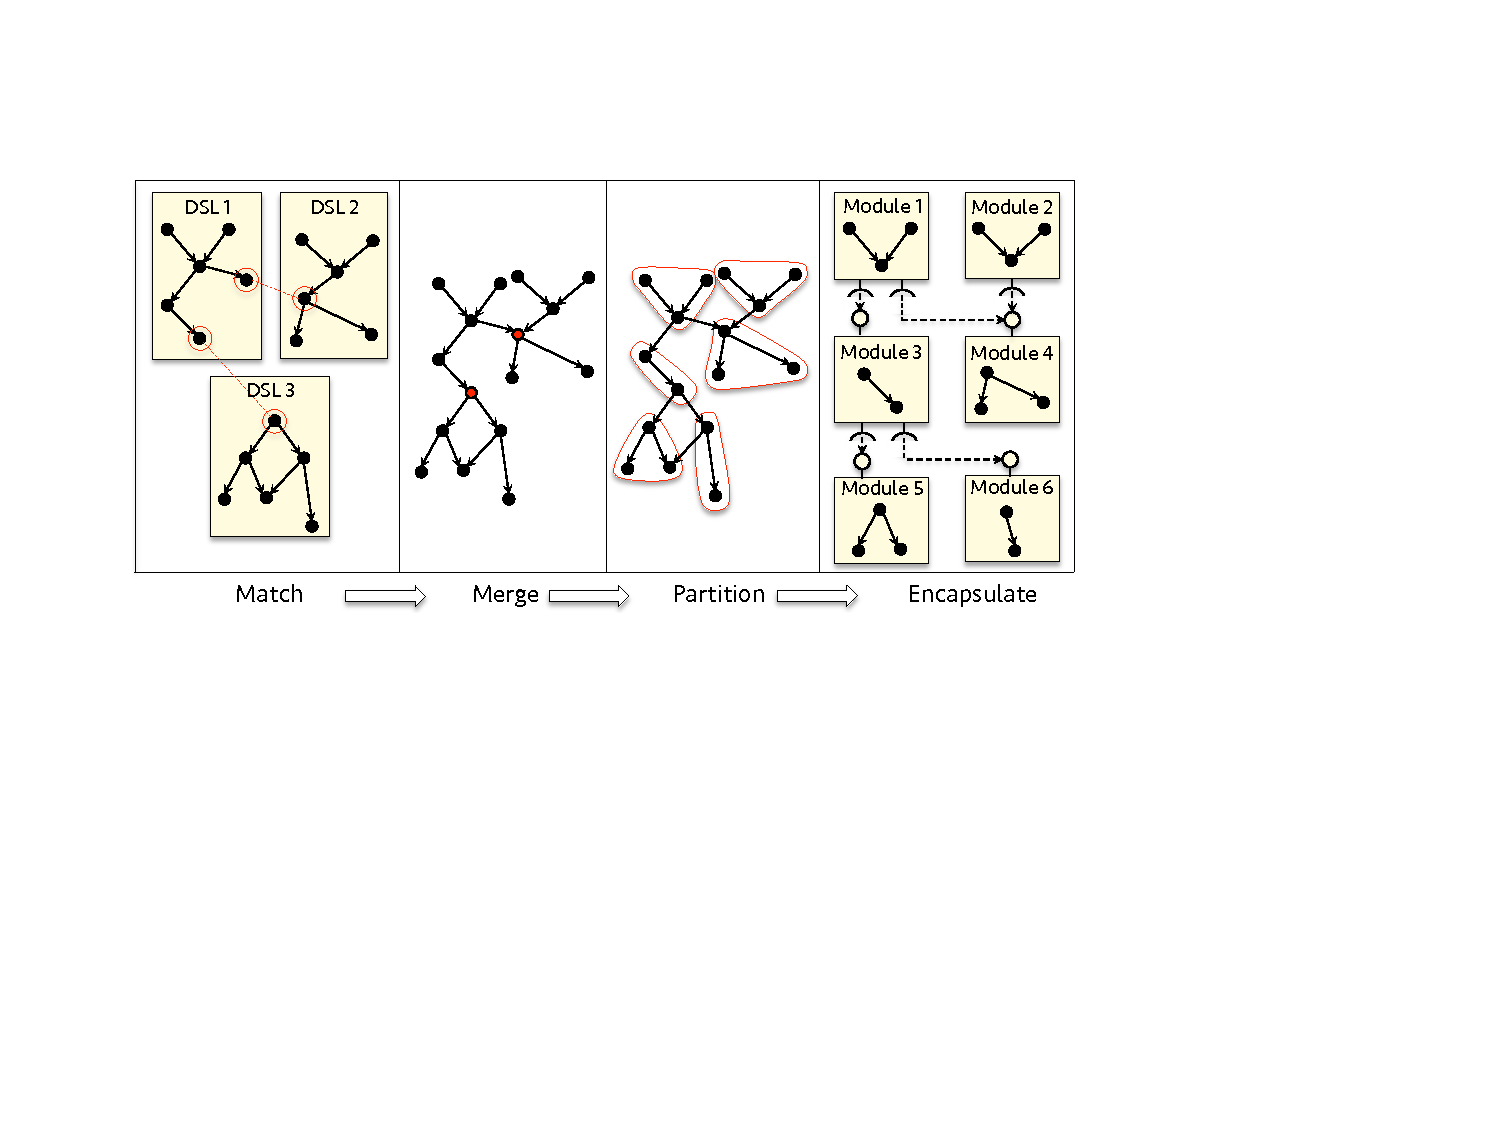
\includegraphics[width=1\linewidth]{images/breaking-down.pdf}
\caption{Process for breaking down a set of DSLs}
\label{fig:breaking-down}
\end{figure*}

\subsubsection{Specifying language modules}

Note that both DSLs and modules are, at the end, set of language constructs. Hence, one may think that a module is also a DSL. Although this is technically true, there is a substantial difference between DSLs and modules. A DSL is a closed set of constructs that materializes a complete DSL specification that is ready to be used. Contrariwise, a module is set of constructs whose specification may depend on other constructs defined in other modules. A module can be used (and considered itself as a DSL) as long as their dependencies are fulfilled.

Accordingly, the main requirement for supporting separation of features in DSLs relies on the capability of expressing dependencies between language modules. In this context, we have identified two types of dependencies: \textit{aggregation} and \textit{extension}. In the following, we explain each of them and we present the corresponding tool support.

\textbf{Language modules \textit{aggregation}:} In aggregation, there is a \textit{requiring module} that \underline{uses} some constructs provided by a \textit{providing module}. The requiring module has a dependency relationship towards the providing one that, in the small, is materialized by the fact that some of the classes of the requiring module have references (simple references or containment references) to some constructs of the providing one.

In order to avoid direct references between modules, we introduce the notion of interfaces for dealing with modules' dependencies. In the case of aggregation, the requiring language has a \textit{required interface} whereas the providing one has the \textit{provided interface}. A required interface contains the set of constructs required by the requiring module which are supposed to be replaced by actual construct provided by other module(s).

It is important to highlight that we use \textit{model types} \cite{Steel:2007} to express both required and provided interfaces. As illustrated on top of Figure \ref{fig:approaches-interfaces}, the relationship between a module and its required interface is \textit{referencing}. A module can have some references to the constructs declared in its required interface. In turn, the relationship between a module and its provided interface is \textit{implements} (deeply explained in \cite{Degueule:2015}). A module implements the functionality exposed in its model type. If the required interface is a subtype of the provided interface, then the provided interface fulfills the requirements declared in a required interface. Note that the partial sub-typing relationship defined in \cite{Guy:2012}, permits a required interface being partially fulfilled by a provided interface. The result of the composition will be a module with a new required interface that contains only those elements that were not provided.


\textbf{Language modules \textit{extension}:} In this case, there is an extension module that (naturally) \underline{extends} the functionality provided by \textit{base module}. The extension module has a dependency to the base module. Moreover, the extension module has little sense by itself without the existence of a base module \cite{Erdweg:2012}. Note that this is a conceptual difference with respect to modules aggregation where the required make sense by itself but requires some external services in order to work correctly.

There are to different mechanisms for extending a base module: \textit{constructs specialization} and \textit{open classes} \cite{Clifton:2000}. In constructs specialization, the constructs of the base module can be extended by adding new subclasses. The extension module contains the new subclasses that reference (by means of the inheritance relationship) the constructs of the base module that are being extended. In this case, the base module remains intact in after the composition but there are additional constructs. In open classes, constructs of the base module can be re-opened and modified by the extension module. For example, for adding a new attribute to a given construct without creating a sub-class, or for overriding a given segment of the semantics. In this case, the extension module is altered after the composition phase. 

Similarly to aggregation, dependencies between the base and the extension modules are specified through interfaces. The base module exposes an \textit{extension point interface} with the constructs that can be extended. In turn, the \textit{extension interface} declares the constructs of the base module that are being extended.

Like in aggregation, and as illustrated at the bottom of Figure \ref{fig:approaches-interfaces}, we use model types of expressing these interfaces. Although the approach is quite similar, there is one fundamental difference between the interfaces in aggregation and the interfaces in extension: the relationship between an extension module and its extension interface is \textit{usage} more than just referencing. That means that the module can to reference the elements declared in the required interface and also modify them by adding new elements. This capability is introduced to support extension by the open-classes mechanism.

\begin{figure*}
\centering
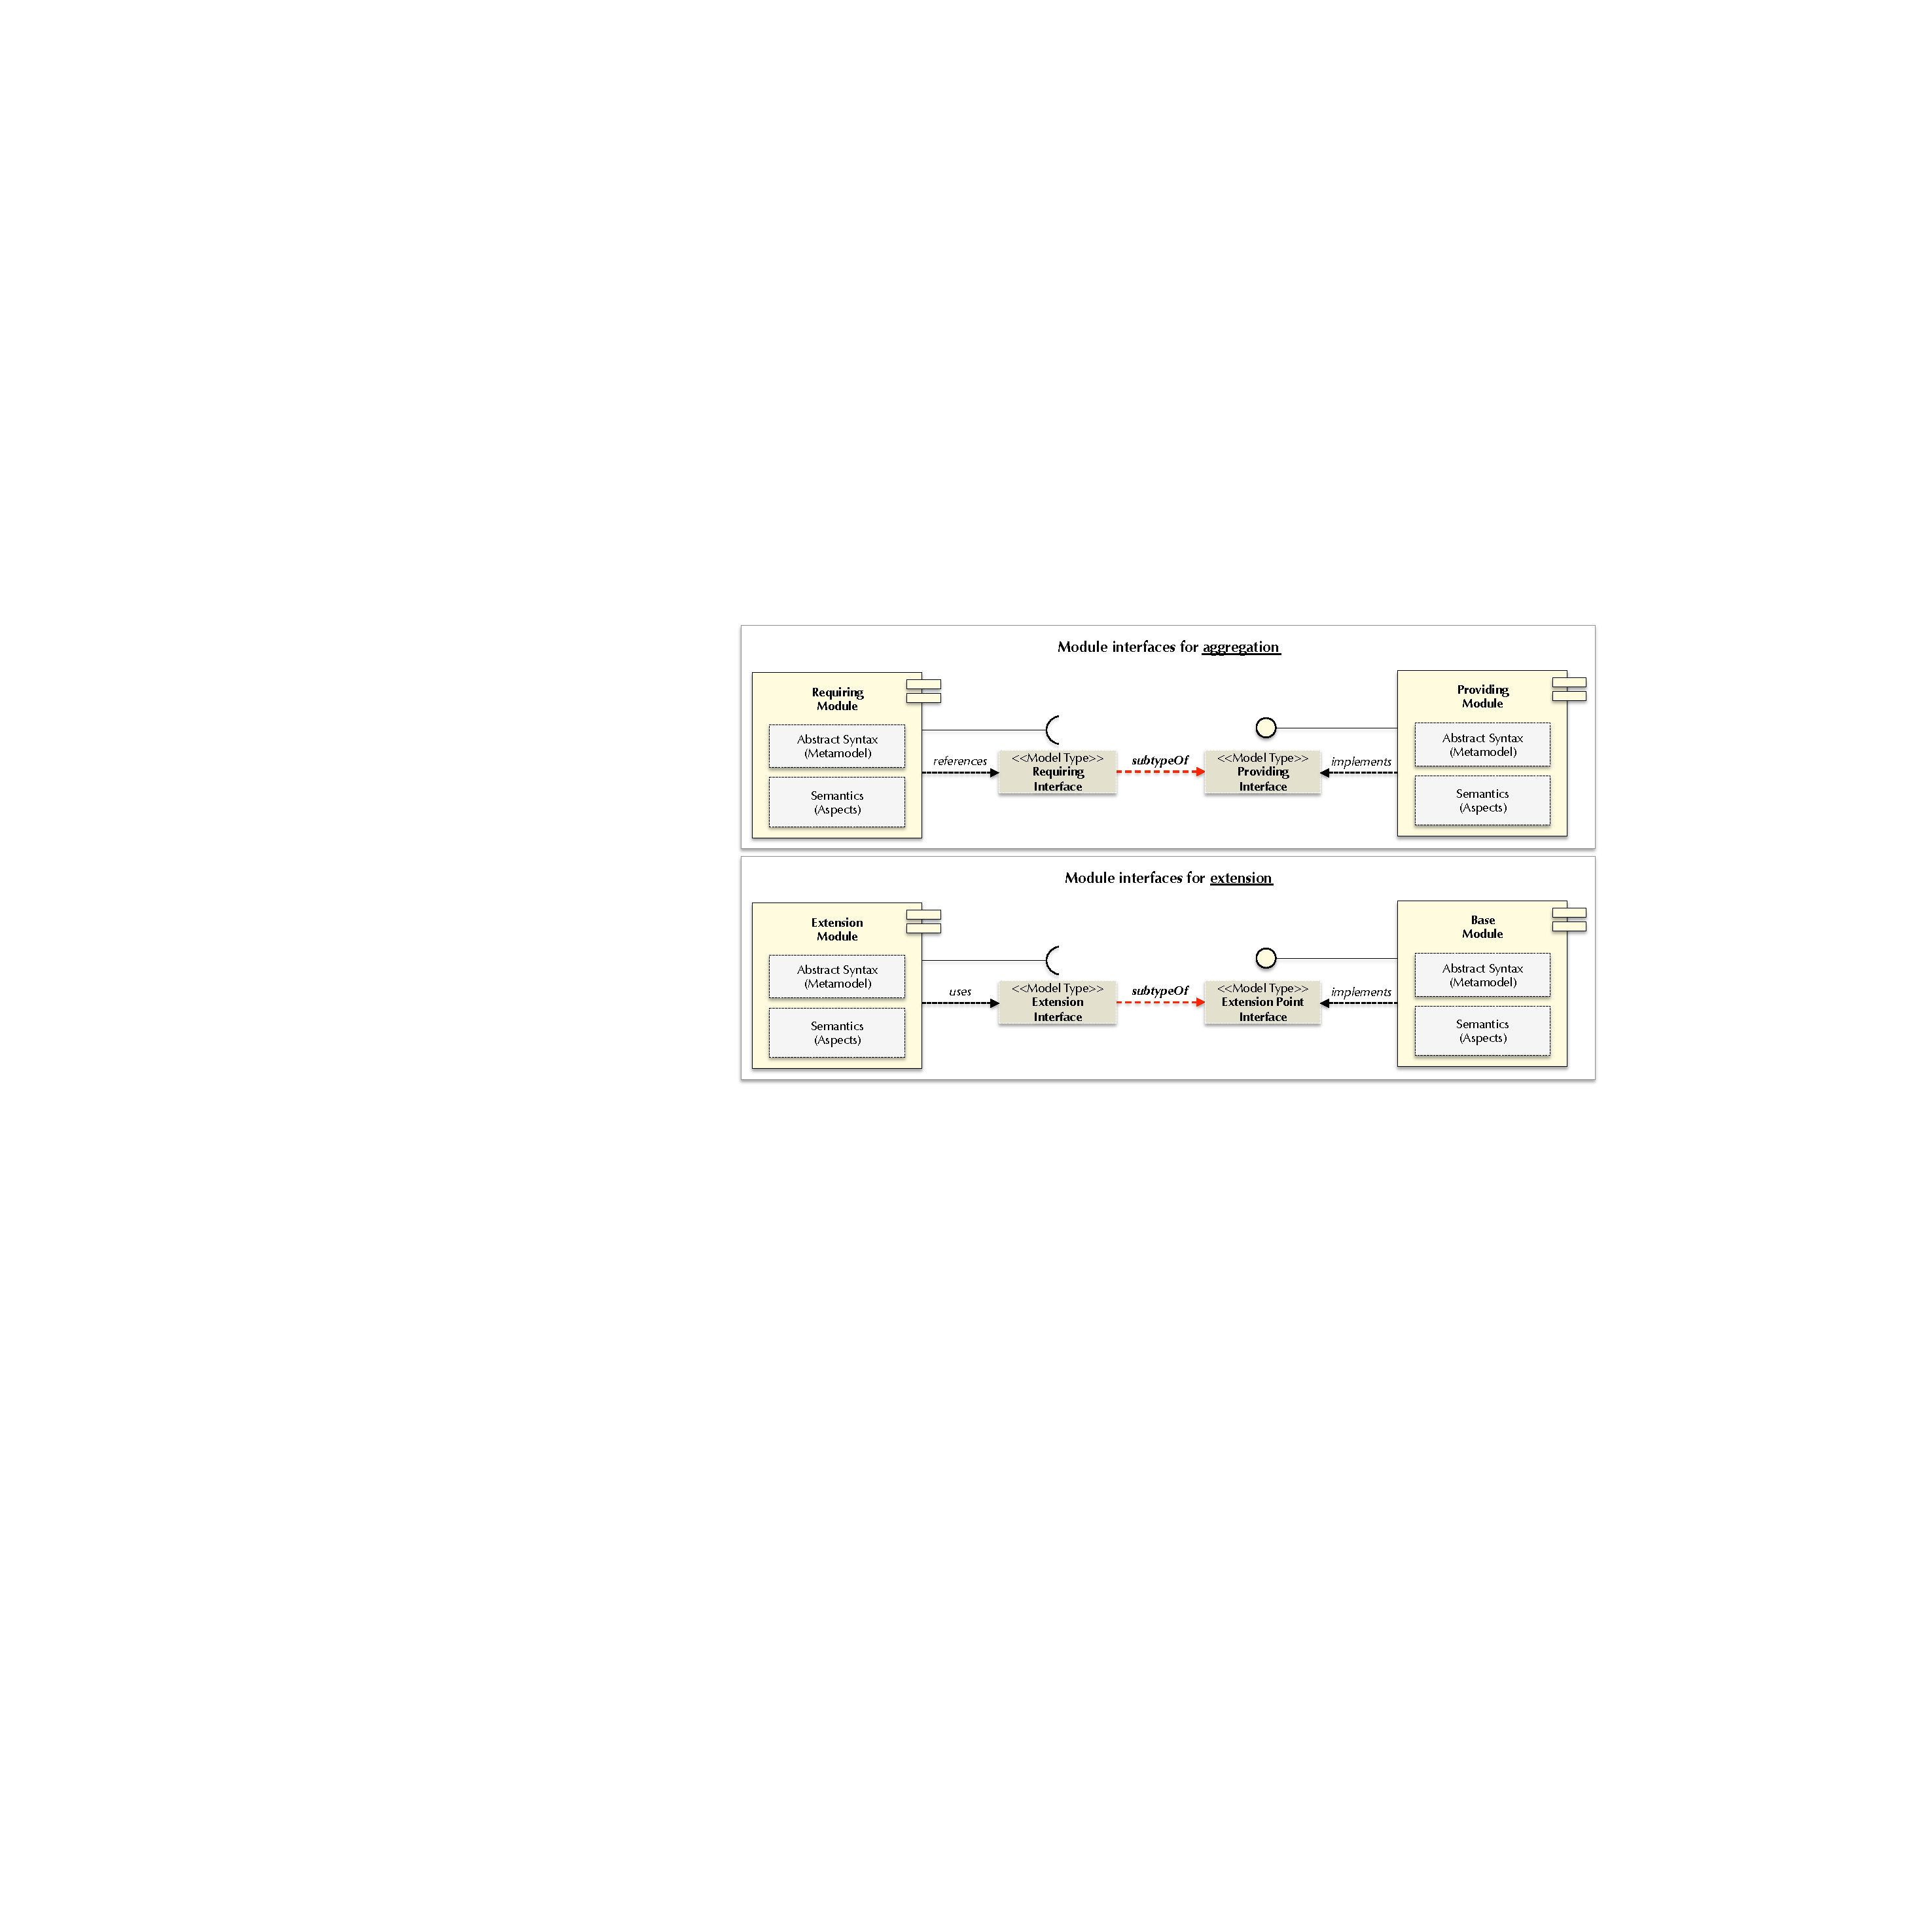
\includegraphics[width=1\linewidth]{images/approaches-interfaces.pdf}
\caption{Interfaces for modularization of DSLs}
\label{fig:approaches-interfaces}
\end{figure*}

\subsection{Inferring the variability model}

After having a set of language modules with their corresponding references among them, we need to automatically infer a variability model that represents the existing variability. To do so, we use as input an algorithm that, based on the dependencies graph of the modules, infer a simple variability model. 



\subsection{Deriving a DSL}

Once the variability of the language product line is correctly specified, the next step is to configure DSLs by using the variability model. Since the variability model is expressed in CVL, the configuration of the language product corresponds to the specification of a realization model that captures the decisions made by the language designers that are configuring the DSL. Our approach uses the realization model to produce the corresponding Melange script. 

As an example, consider the configuration presented in the variability model of the Figure \ref{fig:multi-dimensional-variability}. The corresponding Melange script is presented in the following listing code snippet:

\begin{lstlisting}
language ModuleA {
   ecore MetamodelA.ecore
   with package.A.Semantics6
}

language ModuleB {
   ecore MetamodelB.ecore
   with package.B.Semantics4
}

language MyDSL {
   aggregation(ModuleB, ModuleA)
}
\end{lstlisting}

Note that the Melange script only contains the language elements that correspond to a given configuration. For example, the ModuleA contains only the Semantics6 because it was the choice made at configuration time. Similarly, ModuleB only contains Semantics4. Note also that there is a third language appearing in the script: MyDSL. This language represents the composition of the language modules and can be understood as the root of the script. In this case, this statement of Melange indicates that the modules A and B are composed by aggregation. The first element in the operation corresponds to the requiring module and the second element corresponds to the providing module. 

Once the configuration process produces a Melange script that captures the choices made by the language designers for a particular DSL, it is necessary to compose the declared language modules and produce the DSL. The composition of a set of modules requires a previous phase of compatibility checking. Not all language modules are compatible and in that case composition cannot be performed. In our approach, check the compatibility of two language modules is to verify the sub-typing relationship between the required and provided interface (for the case of aggregation), and the extension and extension point interfaces (for the case of extension).

Once this compatibility checking is correctly verified, language modules are composed. In particular, their specifications are be merged to generate a complete language specification. This merging basically replaces the elements of the required interface by its corresponding implementation in the provided component. A similar process is performed in the case of extension. 

\section*{Acknowledgments}
The research presented in this paper is supported by the European Union within the FP7 Marie Curie Initial Training Network ``RELATE" under grant agreement number 264840 and VaryMDE, a collaboration between Thales and INRIA.

% BIBLIOGRAPHY
\bibliographystyle{abbrv}
\bibliography{0-main}

\end{document}
